\documentclass[aspectratio=169]{beamer}
\usetheme[
    faculty=tsr,
    logo=tsrbeamer/logo/mu/testBackground.png % Custom logo
]{tsrbeamer}
\usepackage[utf8]{inputenc}
\usepackage[main=english]{babel}

%% These macros specify information about the presentation
\title{Coding Workshop}
\subtitle{Creating Your Online Presence}
\author{Mathijs de Jong}

%% These additional packages are used within the document:
\usepackage{ragged2e}  % `\justifying` text
\usepackage{booktabs}  % Tables
\usepackage{tabularx}
\usepackage{tikz}      % Diagrams
\usetikzlibrary{calc, shapes, backgrounds}
\usepackage{amsmath, amssymb}
\usepackage{url}       % `\url`s
\usepackage{hyperref}
\usepackage{listings}  % Code listings
\usepackage{geometry}
\usepackage{soul}
\usepackage{listings}
\usepackage{parcolumns}
\frenchspacing

\setcounter{tocdepth}{1}
\lstdefinelanguage{JavaScript}{
  keywords={typeof, new, true, false, catch, function, return, null, catch, switch, var, if, in, while, do, else, case, break},
  keywordstyle=\color{red}\bfseries,
  ndkeywords={class, export, boolean, throw, implements, import, this},
  ndkeywordstyle=\color{white}\bfseries,
  identifierstyle=\color{yellow},
  sensitive=false,
  comment=[l]{//},
  morecomment=[s]{/*}{*/},
  commentstyle=\color{purple}\ttfamily,
  stringstyle=\color{green}\ttfamily,
  morestring=[b]',
  morestring=[b]"
}


\newenvironment{backgroundframe}[2]{
    \usebackgroundtemplate{\includegraphics[width=\paperwidth]{resources/TSR_background_#2.pdf}}
    \begin{frame}{#1}
}{
    \end{frame}
}

\begin{document}

    {
        \usebackgroundtemplate{
\includegraphics[width=\paperwidth]{resources/TSR_background_6.pdf}}
        \frame{\maketitle}
    }
    
    \begin{darkframes}
    
    \begin{frame}{Outline of the Workshop}
        \frametitle{Outline of the Presentation}
        \tableofcontents
    \end{frame}
    
    \section{Introduction}
    \begin{frame}{What is Web Development?}
        \begin{itemize}
            \item The work involved in developing a web site for the internet or an intranet.
            \item Three kinds of web developer specializations:
            \begin{itemize}
                \item Front-end developer
                \item Back-end developer
                \item Full-stack developer
            \end{itemize}
            \item Our focus: font-end development
        \end{itemize}
    \end{frame}
    
    \section{Installing Basic Software}
    \begin{frame}{Installing Basic Software}
        \begin{itemize}
            \item Requirements:
            \begin{itemize}
                \item A computer
                \item A text editor
                \begin{itemize}
                    \item \href{https://www.sublimetext.com/3}{Sublime Text 3}
                    \item Notepad (Windows)
                    \item \href{https://flight-manual.atom.io/getting-started/sections/installing-atom/}{Atom}
                    \item \href{https://notepad-plus-plus.org/download/v7.6.4.html}{Notepad++}
                \end{itemize}
                \item A web browser
                \begin{itemize}
                    \item \href{https://support.google.com/chrome/answer/95346?co=GENIE.Platform\%3DDesktop\&hl=en}{Google Chrome}
                    \item \href{https://www.mozilla.org/en-US/firefox/new/}{Mozilla Firefox}
                    \item Microsoft Edge
                \end{itemize}
                \item A graphics editor
                \begin{itemize}
                    \item \href{https://www.gimp.org/downloads/}{GIMP}
                    \item Adobe Photoshop
                    \item Sketch
                \end{itemize}
            \end{itemize}
        \end{itemize}
    \end{frame}
    
    \section{What Will Your Website Look Like?}
    \begin{frame}{What Will Your Website Look Like?}
        \begin{itemize}
            \item Before you start writing the code, you should plan it first
            \begin{enumerate}
                \item What is your website about?
                \item What information are you presenting on the subject?
                \item What does your website look like?
            \end{enumerate}
            \item Next, grab pen and paper and sketch out roughly how you want your site to look
            \item \textbf{TIP:} Use templates!
        \end{itemize}
    \end{frame}
    
    \section{Dealing with Files}
    \begin{frame}{Dealing with Files}
        \begin{itemize}
            \item Create a folder for your website
            \item Inside the folder you should include:
            \begin{enumerate}
                \item \textit{\textbf{index.html}}: This file will generally contain your homepage content, that is, the text and images that people see when they first go to your site.
                \item \textit{\textbf{images} folder}: This folder will contain all the images that you use on your site.
                \item \textit{\textbf{styles} folder}: This folder will contain the CSS code used to style your content.
                \item \textit{\textbf{scripts} folder}: This folder will contain all the JavaScript code used to add interactive functionality to your site.
            \end{enumerate}
        \end{itemize}
    \end{frame}

    \defverbatim[colored]\firstWebPage{
      \begin{lstlisting}[language=HTML,tabsize=2, basicstyle=\tiny, xleftmargin=.2\textwidth]
<!DOCTYPE html>
<html>
  <head>
    <meta charset="utf-8">
    <title>My test page</title>
  </head>
  <body>
    <h3>Hello World!</h3>
  </body>
</html>
    \end{lstlisting}}
    
    \begin{frame}{Creating Your First Website}
        \begin{enumerate}
            \item Open up your \textit{index.html} file, and insert the following code into the file exactly as shown.
            \firstWebPage
            \item Save your HTML file, then load it in your web browser (double-click the file). You should see your new web page displaying "Hello World!". 
        \end{enumerate}
    \end{frame}
    
    \section{HTML Basics}
    \begin{frame}{HTML — HTML Basics}
    \begin{itemize}
        \item \textbf{H}yper\textbf{t}ext \textbf{M}arkup \textbf{L}anguage
        \item Structure a web page and its content
        \item A \st{programming} markup language
        \item Series of elements that enclose, or wrap, different parts of content to make it appear or act a certain way.
    \end{itemize}
    \end{frame}
    
    \begin{frame}{HTML — Anatomy of an HTML Element}
        \begin{figure}[h]
            \centering
            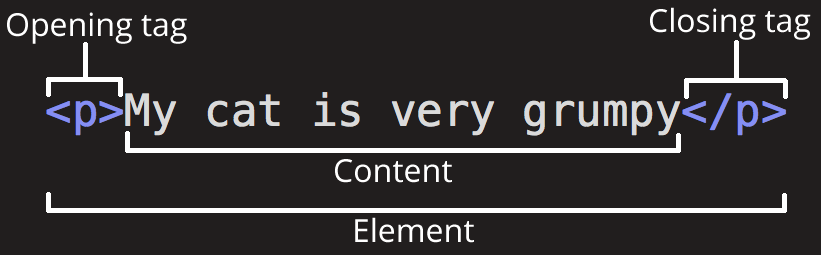
\includegraphics[width=0.5\linewidth]{resources/grumpy-cat-small.png}
        \end{figure}
        \begin{enumerate}
            \item \textbf{The opening tag:} This consists of the name of the element (in this case, p), wrapped in opening and closing angle brackets. This states where the element begins or starts to take effect.
            \item \textbf{The closing tag:} This is the same as the opening tag, except that it includes a \textit{forward slash} before the element name. This states where the element ends.
            \item \textbf{The content:} This is the content of the element, which in this case is just text.
            \item \textbf{The element:} The opening tag, the closing tag, and the content together comprise the element.
        \end{enumerate}
    \end{frame}
    
    \begin{frame}{HTML — Attributes}
        \begin{figure}[h]
            \centering
            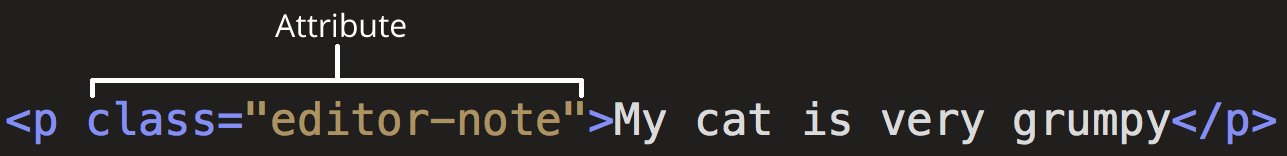
\includegraphics[width=0.7\linewidth]{resources/grumpy-cat-attribute-small.png}
        \end{figure}
        \begin{itemize}
            \item Attributes contain extra information about the element that you don't want to appear in the actual content
            \item \textit{class} is the attribute \textit{name}
            \item \textit{editor-note} is the attribute \textit{value}
        \end{itemize}
    \end{frame}
    
    \begin{frame}{HTML — Anatomy of an HTML Document}
        \firstWebPage
        \begin{itemize}
            \item \textit{<!DOCTYPE html>} — The doctype.
        \end{itemize}
    \end{frame}
    
    \begin{frame}{HTML — Anatomy of an HTML Document}
        \firstWebPage
        \begin{itemize}
            \item \textit{<html></html>} — This element wraps all the content on the entire page and is sometimes known as the root element.
        \end{itemize}
    \end{frame}
    
    \begin{frame}{HTML — Anatomy of an HTML Document}
        \firstWebPage
        \begin{itemize}
            \item \textit{<head></head>} — This element acts as a container for all the stuff you want to include on the HTML page that isn't the content you are showing to your page's viewers.
        \end{itemize}
    \end{frame}
    
    \begin{frame}{HTML — Anatomy of an HTML Document}
        \firstWebPage
        \begin{itemize}
            \item \textit{<meta charset="utf-8">} — This element sets the character set your document should use to UTF-8, which includes most characters from the vast majority of written languages.
        \end{itemize}
    \end{frame}
    
    \begin{frame}{HTML — Anatomy of an HTML Document}
        \firstWebPage
        \begin{itemize}
            \item \textit{<title></title>} — This sets the title of your page, which is the title that appears in the browser tab the page is loaded in.
        \end{itemize}
    \end{frame}
    
    \begin{frame}{HTML — Anatomy of an HTML Document}
        \firstWebPage
        \begin{itemize}
            \item \textit{<body></body>} — This contains all the content that you want to show to web users when they visit your page, whether that's text, images, videos, games, playable audio tracks, or whatever else.
        \end{itemize}
    \end{frame}
        
    \defverbatim[colored]\htmlImage{
      \begin{lstlisting}[language=HTML,tabsize=2]
<img src="images/firefox-icon.png" alt="My test image">
    \end{lstlisting}}
    
    \begin{frame}{HTML — Images}
        \begin{figure}[h]
           \begin{flushleft} 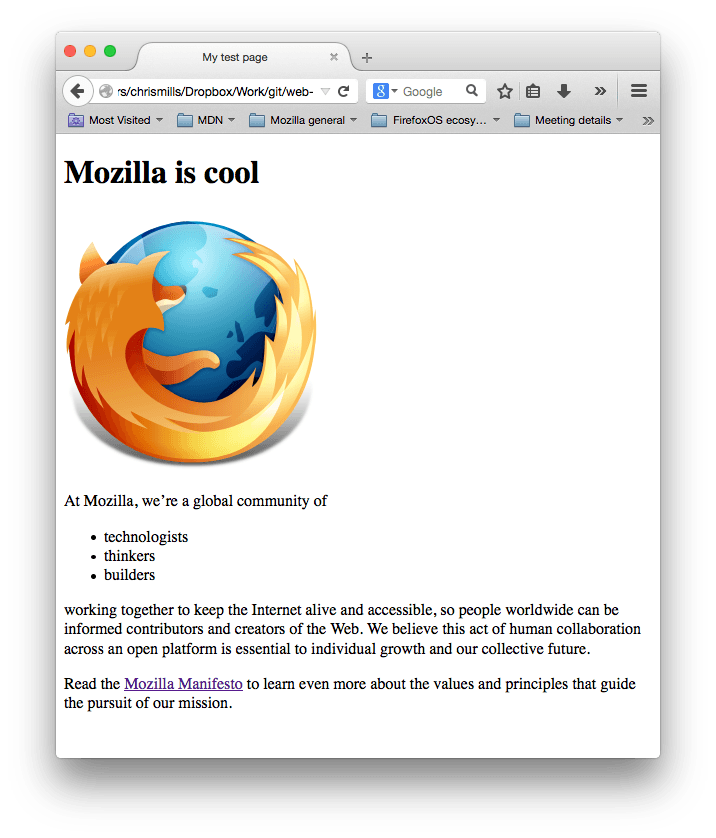
\includegraphics[width=0.35\linewidth]{resources/finished-test-page-small.png}
           \end{flushleft}
        \end{figure}
        \htmlImage
    \end{frame}
    
    \begin{frame}{HTML — Marking Up Text}
        \begin{itemize}
            \item Headings
            \begin{itemize}
                \item Heading elements allow you to specify that certain parts of your content are headings or subheadings.
                \item HTML contains 6 heading levels, \textit{<h1>}–\textit{<h6>}.
            \end{itemize}
            \item Paragraphs
            \begin{itemize}
                \item \textit{<p>} elements are for containing paragraphs of text; you'll use these frequently when marking up regular text content.
            \end{itemize}
            \item Lists
            \begin{itemize}
                \item \textit{Unordered lists} are for lists where the order of the items doesn't matter, such as a shopping list. These are wrapped in a \textit{<ul>} element.
                \item \textit{Ordered lists} are for lists where the order of the items does matter, such as a recipe. These are wrapped in an \textit{<ol>} element.
                \item Each item inside the lists is put inside an \textit{<li>} (list item) element.
            \end{itemize}
        \end{itemize}
    \end{frame}
    
    \defverbatim[colored]\htmlLink{
      \begin{lstlisting}[language=HTML,tabsize=2]
<a href="https://www.mozilla.org/en-US/about/manifesto/">Mozilla Manifesto</a>
    \end{lstlisting}}
    
    \begin{frame}{HTML — Links}
        \begin{itemize}
            \item To add a link, we need to use a simple element — \textit{<a>} — "a" being the short form for "anchor".
            \item To make text within your paragraph into a link, follow these steps:
            \begin{enumerate}
                \item Choose some text. We chose the text "Mozilla Manifesto".
                \item Wrap the text in an <a> element.
                \item Give the <a> element an href attribute.
                \item Fill in the value of this attribute with the web address that you want the link to link to:
            \end{enumerate}
            \htmlLink
        \end{itemize}
    \end{frame}
    
    \begin{frame}{HTML - Marking up a Letter Exercise}
        \begin{itemize}
            \item Now that you are familiar with HTML, you can start practicing with it
            \item Before you get started, you might want to read the \href{https://developer.mozilla.org/en-US/docs/Learn/Getting_started_with_the_web/HTML_basics}{HTML Basics} article
            \item Try to work on the \href{https://developer.mozilla.org/en-US/docs/Learn/HTML/Introduction_to_HTML/Marking_up_a_letter}{marking up a letter exercise}
            \item Check out the articles in the \href{https://developer.mozilla.org/en-US/docs/Learn/HTML}{HTML — Structuring the Web} section to find more detailed explanations on how to solve the marking up a letter exercise
        \end{itemize}
    \end{frame}
    
    \section{CSS Basics}
    \begin{frame}{CSS — CSS Basics}
    \begin{itemize}
        \item \textbf{C}ascading \textbf{S}tyle \textbf{S}heets
        \item Code used to style your web page
        \item A \st{programming} \st{markup} style sheet language
        \item Used to apply styles selectively to elements in HTML documents
    \end{itemize}
    \end{frame}
    
    \defverbatim[colored]\cssExternalHtml{
      \begin{lstlisting}[language=HTML,tabsize=2, basicstyle=\tiny, xleftmargin=.1\textwidth]
<!DOCTYPE html>
<html>
  <head>
    <meta charset="utf-8">
    <title>My CSS experiment</title>
    <link rel="stylesheet" href="style.css">
  </head>
  <body>
    <h1>Hello World!</h1>
    <p>This is my first CSS example</p>
  </body>
</html>
    \end{lstlisting}}
    
    \defverbatim[colored]\cssExternalCss{
      \begin{lstlisting}[language=HTML,tabsize=2, basicstyle=\tiny, xleftmargin=.4\textwidth]
h1 {
  color: blue;
  background-color: yellow;
  border: 1px solid black;
}

p {
  color: red;
}
    \end{lstlisting}}
    
    \begin{frame}{CSS — Apply Your CSS to Your HTML}
        \begin{enumerate}
            \item External stylesheet
        \end{enumerate}
        \cssExternalHtml
        \cssExternalCss
    \end{frame}

    \defverbatim[colored]\cssInternal{
      \begin{lstlisting}[language=HTML,tabsize=2, basicstyle=\tiny, xleftmargin=.1\textwidth]
<!DOCTYPE html>
<html>
  <head>
    <meta charset="utf-8">
    <title>My CSS experiment</title>
    <style>
      h1 {
        color: blue;
        background-color: yellow;
        border: 1px solid black;
      }

      p {
        color: red;
      }
    </style>
  </head>
  <body>
    <h1>Hello World!</h1>
    <p>This is my first CSS example</p>
  </body>
</html>
    \end{lstlisting}}

    \begin{frame}{CSS — Apply Your CSS to Your HTML}
        \begin{enumerate}
            \item [2.] Internal stylesheet
        \end{enumerate}
        \cssInternal
    \end{frame}
    
\defverbatim[colored]\cssInline{
      \begin{lstlisting}[language=HTML,tabsize=2, basicstyle=\tiny, xleftmargin=.1\textwidth]
<!DOCTYPE html>
<html>
  <head>
    <meta charset="utf-8">
    <title>My CSS experiment</title>
  </head>
  <body>
    <h1 style="color: blue;background-color: yellow;border: 1px solid black;">Hello World!</h1>
    <p style="color:red;">This is my first CSS example</p>
  </body>
</html>
    \end{lstlisting}}
    \begin{frame}{CSS — Apply Your CSS to Your HTML}
        \begin{enumerate}
            \item [3.] Inline styles
        \end{enumerate}
        \cssInline
    \end{frame}

    \begin{frame}{CSS — Anatomy of a CSS Ruleset}
        \begin{figure}[h]
            \centering
            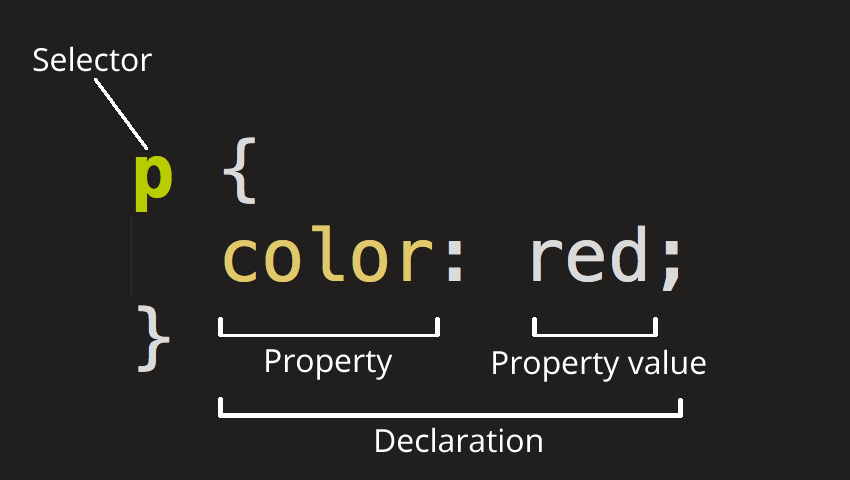
\includegraphics[width=0.4\linewidth]{resources/css-declaration-small.png}
        \end{figure}
        \begin{itemize}
            \item The whole structure is called a \textit{rule set}
            \item \textit{Selector} — Selects the element(s) to be styled
            \item \textit{Declaration} — Specifies which of the element's properties you want to style
            \item \textit{Properties} — Ways in which you can style a given HTML element
            \item \textit{Property value} — Chooses one out of many possible appearances for a given property
        \end{itemize}
    \end{frame}
    
    \begin{frame}{CSS — Different Types of Selectors}
        \begin{figure}[h]
            \begin{flushleft}
            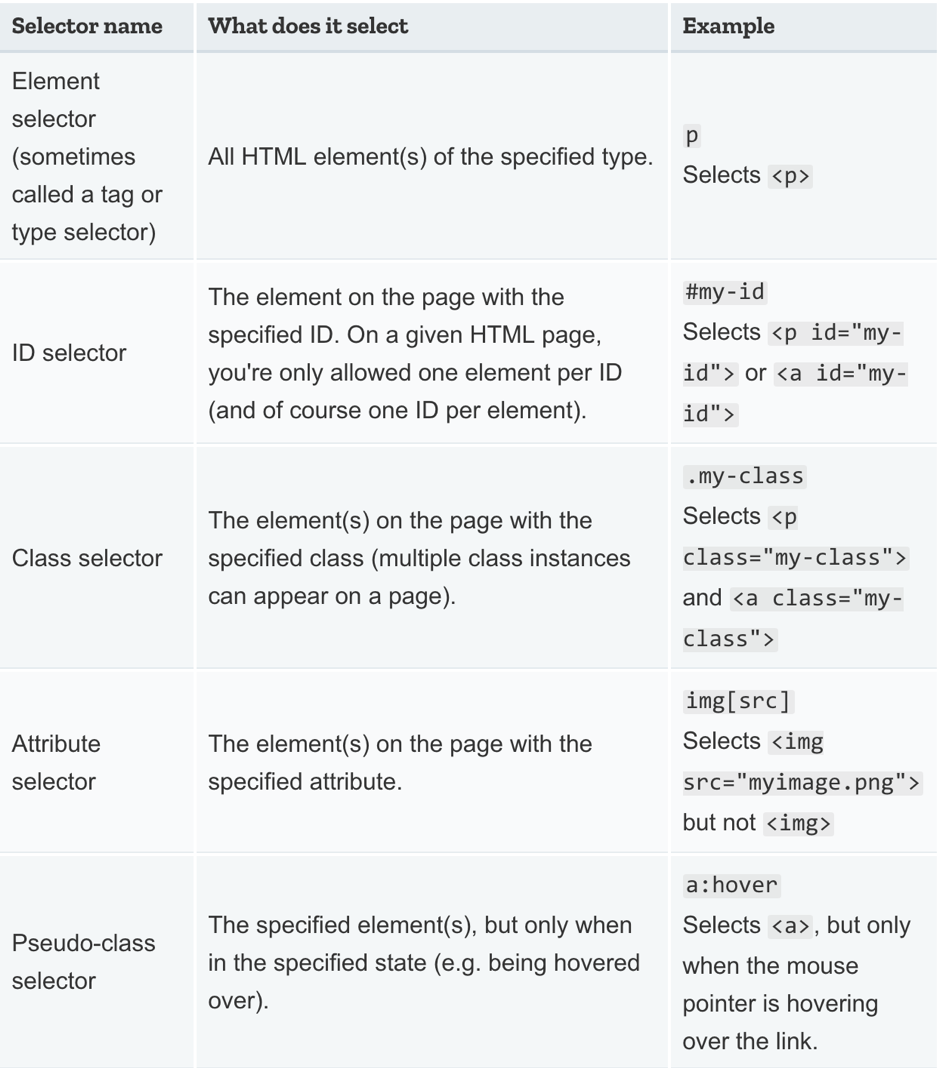
\includegraphics[width=0.4\linewidth]{resources/css-different-selectors.png}
            \end{flushleft}
        \end{figure}
    \end{frame}
    
    \begin{frame}{CSS — Boxes, Boxes Everywhere}
        \begin{figure}[h]
            \centering
            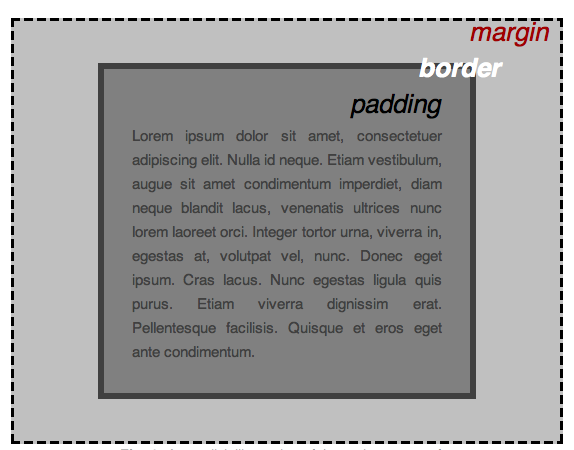
\includegraphics[width=0.35\linewidth]{resources/box-model.png}
        \end{figure}
        \begin{itemize}
            \item CSS layour is based principally on the \textit{box model}
            \item Each of the blocks taking up space on your page has properties like this:
            \begin{itemize}
                \item \textit{padding} — the space just around the content
                \item \textit{border} — the solid line that sits just outside the padding
                \item \textit{margin} — the space around the outside of the element
            \end{itemize}
        \end{itemize}
    \end{frame}
    
    \begin{frame}{CSS — Style Your Page Exercise}
        \begin{itemize}
            \item Now that you are familiar with CSS, you can start practicing with it
            \item Before you get started, you might want to read the \href{https://developer.mozilla.org/en-US/docs/Learn/Getting_started_with_the_web/CSS_basics}{CSS Basics} article
            \item Try to work your way through the \href{https://www.w3schools.com/css/exercise.asp}{W3School CSS exercises}
            \item Check out the articles in the \href{https://developer.mozilla.org/en-US/docs/Learn/CSS}{CSS — Styling the Web} section to find more detailed explanations on how to solve the CSS exercises
        \end{itemize}
    \end{frame}
    
    \section{JavaScript Basics}
    
    \defverbatim[colored]\jsExternalScript{
      \begin{lstlisting}[language=JavaScript,tabsize=2, xleftmargin=.1\textwidth]
<script src="scripts/main.js"></script>
    \end{lstlisting}}
    
     \begin{frame}{JavaScript — Make Your Web Page Dynamic}
        \begin{itemize}
            \item Programming language that adds interactivity to your website
            \item Much more powerful and complexer than HTML and CSS
            \item External script
            \jsExternalScript
            \item Learn by doing with the \href{https://www.codecademy.com/learn/introduction-to-javascript}{CodeAcademy — Introduction To JavaScript} course
        \end{itemize}
        
    \end{frame}
    
    \begin{frame}{Time to Start Working on Your Own Website}
        Time to start working on your own project! However, before you get started, you might want to go over the following articles.
        \begin{enumerate}
            \item \href{https://developer.mozilla.org/en-US/docs/Learn/Getting_started_with_the_web/What_will_your_website_look_like}{What will your website look like?}
            \item \href{https://developer.mozilla.org/en-US/docs/Learn/Getting_started_with_the_web/Dealing_with_files}{Dealing with files}
            \item \href{https://developer.mozilla.org/en-US/docs/Learn/Getting_started_with_the_web/HTML_basics}{HTML basics}
            \item \href{https://developer.mozilla.org/en-US/docs/Learn/Getting_started_with_the_web/CSS_basics}{CSS basics}
            \item \href{https://developer.mozilla.org/en-US/docs/Learn/Getting_started_with_the_web/JavaScript_basics}{JavaScript Basics}
            \item \href{https://developer.mozilla.org/en-US/docs/Learn/Getting_started_with_the_web/Publishing_your_website\#Publishing_via_GitHub}{Publishing via Github}
            \item \href{https://developer.mozilla.org/en-US/docs/Learn/JavaScript/First_steps/A_first_splash}{JavaScript — A splash into JavaScript}
            \item \href{https://developer.mozilla.org/en-US/docs/Learn/Getting_started_with_the_web/How_the_Web_works}{How the Web works}
        \end{enumerate}
    \end{frame}
    
    \begin{frame}{Make Your Own Personal Website}
        \begin{itemize}
            \item That's it! Now you know how the Web works and how you can add your content to it
            \item What better way to do this than by creating your own personal website?
            \item You can check out the following links for inspiration:
            \begin{itemize}
                \item \href{https://medium.muz.li/25-best-personal-website-design-examples-and-resources-for-your-inspiration-446f7ac0bb71}{Medium — 25 Best Personal Website Design Examples and Resources for Your Inspiration}
                \item \href{https://www.awwwards.com/websites/portfolio/}{Portfolio — Best Portfolio Websites}
            \end{itemize}
            \item \textit{TIP:} Start simple and work in sprints!
        \end{itemize}
    \end{frame}
    
    \end{darkframes}
\end{document}
